\section{\Compose* Architecture}
\label{sec:TheComposestarArchitecture}
\begin{figure}
  \centering
  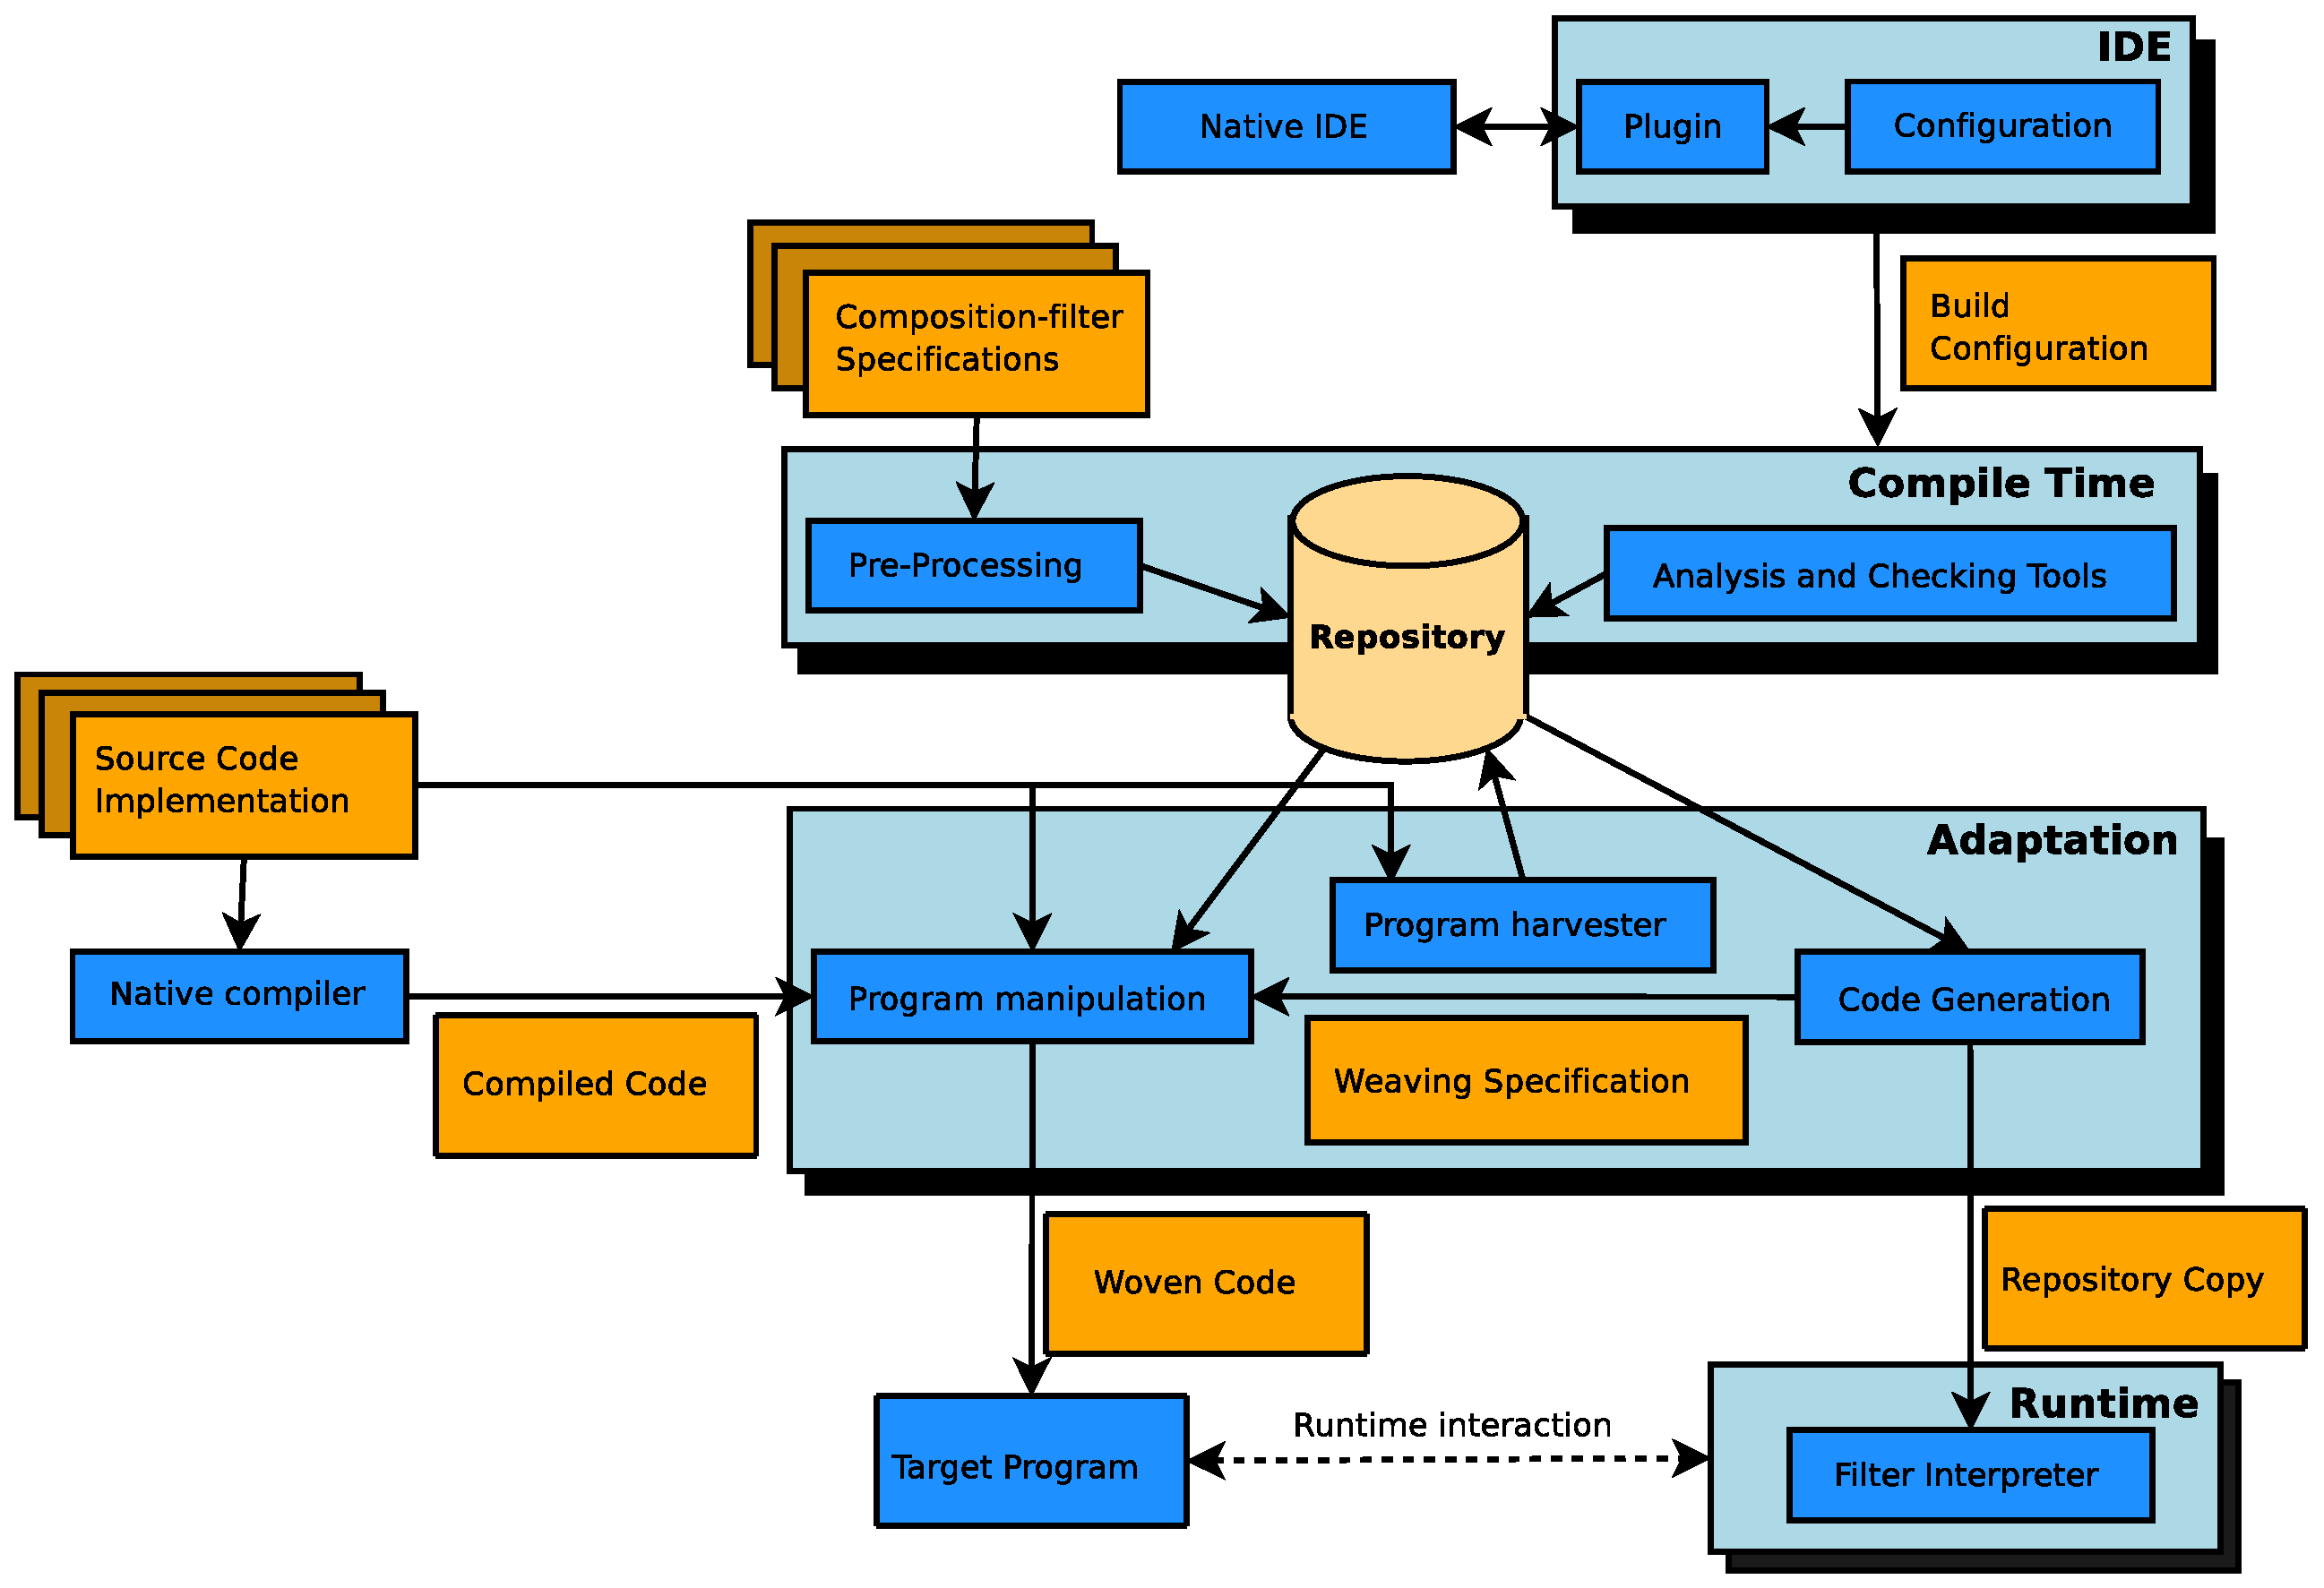
\includegraphics[style=halfheight]{Architecture05}
  \caption[Overview of the \Compose* architecture]{%
    Overview of the \Compose* architecture}
  \label{fig:ComposestarArchitecture}
\end{figure}
An overview of the \Compose* architecture is illustrated in \autoref{fig:ComposestarArchitecture}.
The \Compose* architecture can be divided in four layers~\cite{Nagy2006}: IDE, compile time, adaptation, and runtime. 

\subsection{Integrated Development Environment}
Some of the purposes of the Integrated Development Environment (IDE) layer are to interface with the native IDE and to create a build configuration.
In the build configuration it is specified which source files and settings are required to build a \Compose* application.
After creating the build configuration the compile time is started.

The creation of a build configuration can be done manually or by using a plug-in.
Examples of these plug-ins are the Visual Studio add-in for \Compose*[.NET] and the Eclipse plug-in for \Compose*[J] and \Compose*[C].

\subsection{Compile Time}
The compile time layer is platform independent and reasons about the correctness of the composition filter implementation with respect to the program which allows the target program to be build by the adaptation.

The compile time `pre-processes' the composition filter specifications by parsing the specification, resolving the references, and checking its consistency.
To provide an extensible architecture to facilitate this process a blackboard architecture is chosen.
This means that the compile time uses a general knowledgebase that is called the `repository'.
This knowledgebase contains the structure and metadata of the program which different modules can execute their activities on.
Examples of modules within analysis and validation are the three modules SANE, LOLA and FILTH.
These three modules are responsible for (some) of the analysis and validation of the super imposition and its selectors.

\subsection{Adaptation}
The adaptation layer consists of the program manipulation, harvester, and code generator.
These components connect the platform independent compile time to the target platform.
The harvester is responsible for gathering the structure and the annotations within the source program and adding this information to the knowledgebase.
The code generation generates a reduced copy of the knowledgebase and the weaving specification.
This weaving specification is then used by the weaver contained by the program manipulation to weave in the calls to the runtime into the target program.
The end result of the adaptation the target program which interfaces wit the runtime.

\subsection{Runtime}
The runtime layer is responsible for executing the concern code at the join points.
It is activated at the join points by function calls that are woven in by the weaver.
A reduced copy of the knowledgebase containing the necessary information for filter evaluation and execution is enclosed with the runtime.
When the function is filtered the filter is evaluated.
Depending on if the the condition part evaluates to true, and the matching part matches the accept or reject behavior of the filter is executed.
The runtime also facilitates the debugging of the composition filter implementations.

\section{Platforms}
The composition filters concept of \Compose* can be applied to any programming language, given that certain assumptions are met.
Currently, \Compose* supports three platforms: \dotNET, Java and C\@.
For each platform different tools are used for compilation and weaving.
They all share the same platform independent compile-time.

\Compose*[.NET] targets the \dotNET platform and is the oldest implementation of \Compose*.
Its weaver operates on CIL byte code.
\Compose*[.NET] is programming language independent as long as the programming language can be compiled to CIL code.
An add-in for Visual Studio is provided for ease of development.
\Compose*[J] targets the Java platform and provides a plug-in for integration with Eclipse.
\Compose*[C] contains support for the C programming language.
The implementation is different from the Java and \dotNET counterparts, because it does not have a run-time environment.
The filter logic is woven directly in the source code.
Because the language C is not based on objects, filters are woven on functions based on membership of sets of functions.
Like the Java platform, \Compose*[C] provides a plug-in for Eclipse.